\documentclass{article}
\usepackage{tikz}
\usetikzlibrary{decorations.markings, shapes}
\definecolor{myyellow}{RGB}{254, 241, 24}
\definecolor{myorange}{RGB}{234, 125, 1}

\begin{document}
\begin{figure}
	\centering
	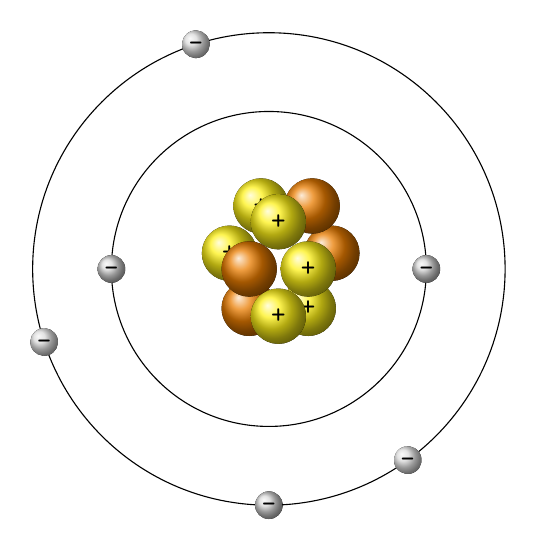
\begin{tikzpicture}
		\def\proton(#1,#2){%
			\fill[shading=ball,ball color=myyellow] (#1,#2) circle (10pt);
			\node at (#1,#2) {\texttt{+}};
	}
	\def\neutron(#1,#2){%
		\fill[shading=ball,ball color=myorange] (#1,#2) circle (10pt);
	}
		\def\electron{%
	\fill[shading=ball,ball color=gray!30] (0,0) circle (5pt);
    \node at (0,0) {\texttt{-}};
	}
	\neutron(0.8,0.2)
	\proton(0.5,-0.5)
	\neutron(-0.25,-0.5)
	\neutron(0.55,0.8)
	\proton(-0.5,0.2)
	\proton(-0.1,0.8)
	\proton(0.5,0)
	\proton(0.12,0.6)
	\proton(0.12,-0.6)
	\neutron(-0.25,0)
		\draw[
		  postaction=decorate,
		  decoration={markings, 
		  mark=at position 0.5 with {\electron},
		  mark=at position 1 with {\electron}
		}] 

		  (0,0) circle (2cm);
		\draw[
			postaction=decorate,
			  decoration={markings, 
		  mark=at position 0.3 with {\electron},
		  mark=at position 0.55 with {\electron},
		mark=at position 0.85 with {\electron},
		mark=at position 0.75 with {\electron}
		}] 
			(0,0) circle (3cm);
		\end{tikzpicture}
	\caption{Drawing the Bohr atomic model}
	\label{}
\end{figure}
\end{document}
